\section{Method}

\subsection{Cloud Infrastructure}
Public cloud being the most preferred choice for enterprise grade application deployments where the microservice communication and security is handed over to Istio, this research is conducted on \acrlong{gcp}. \acrshort{gcp} remains the choice as public cloud provider for this research project mainly because of the author's familiarity with the platform. As Istio works at Kubernetes environment level, all the methods used in this research are conducted on \acrlong{gke} - the fully managed Kubernetes service offered by \acrshort{gcp}.

\subsubsection{High Level Strategy}
To maintain a consistent and steady approach for each deployment and testing stages, \acrfull{iac} is used with Terraform. A rapid cloud infrastructure provisioning and de-provisioning model is followed to keep the cloud cost minimal. All the Terraform IaC, Shell scripts and Kubernetes configurations files used in this research are available at \ref{appendix:researchRepo}. At a high level first the Kubernetes cluster is provisioned and verified by kubectl on local system. Next the observability stack is installed on the cluster followed by the service mesh itself is installed and verified. After all the platform level stuffs are installed, configured and verified, a demo web application \acrfull{boa} is deployed using Kubernetes manifest files including the front end microservice attachment to the Istio ingress controller. This enables the application to be accessed from outside of the cluster. At the end of each testing sessions, everything is teared down completely using \acrshort{iac} to save cloud cost.

\subsubsection{Terraform Provisioning}
Google offers several Terraform APIs to customize the cluster resource provisioning which gives a greater control and flexible management of \acrshort{gke} cluster. As a prerequisite of Terraform provisioninig a GCP project and service account is created manually from \acrshort{gcp} console along with enabling all required APIs using gcloud command line tool on local system. \acrfull{iac} used in this research leverages several Terraform modules to provision the \acrshort{gke} cluster along with necessary cloud components like \acrshort{vpc} network, subnet and node pool. Terraform script defines the following configurations for the cluster creation.
\begin{itemize}
  \item GCP europe-west1-b zonal cluster
  \item e2-standard-2 machine type with 2 vCPU and 8GiB RAM
  \item Latest stable release of Kubernetes v1.27.3
  \item Node scaling from 1 to 10 with an initial count of 2
\end{itemize}

Essentially, a zonal cluster is created in europe-west1 physically located at Belgium (\cite{gcpDocRegion}) to keep the cloud cost to minimal. The default node pool comes with a cluster is not used here to define some custom parameters like manual IP ranges for Kubernetes services and pods, lower disk size. Selecting the machine type as e2-standard-2 gives \acrshort{boa} an ample amount of resources along with Istio components. Kubernetes version is set to v1.27.3 which is one of the most recent and stable release of Kubernetes (\cite{kubeDocRelease}) at the time of writing this paper.


\subsubsection{Demo Application}
\acrshort{boa}, a microservice based demo application from \acrshort{gcp} open source repository \cite{githubBOA} is used for this research project. This application is developed by \acrshort{gcp} team to demonstrate their products and proven to be a perfect fit for evaluating Ambient mesh as it comes with predefined Kubernetes deployment manifest files. With minimal changes to these manifest files, microservice deployment remains fairly straight forward job for the research. This enables focusing more on the Istio rather investing more time on application source code build and deployment. \acrshort{boa} simulates a virtual online banking system with facilities of account opening, deposit, withdraw and balance enquiry. This application consists of a total nine microservices out of which, eight microservices are used without any modifications for this research. The application follows a typical microservice based architecture which is defined in Figure \ref{method:boaDesign}.

\begin{figure}[ht!]
  \centering
  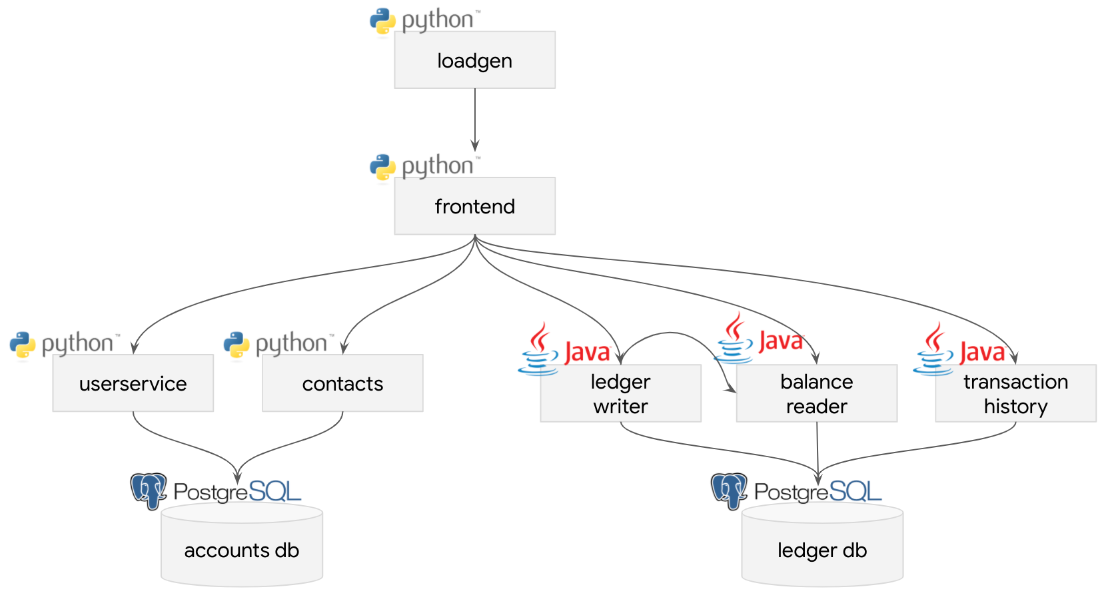
\includegraphics[width=1.0\linewidth]{resources/boa-architecture.png}
  \caption{Bank of Anthos application architecture}
  \label{method:boaDesign}
\end{figure}

The load generator script comes with the project is modified to suite the purpose of this research and run from local system to reduce the burden on the cluster.


\subsection{Observability Mechanism}
\label{observabilityStack}
Monitoring in dynamic service-oriented architectures is a crucial point of success and observability takes it all to a complete new level by exploring the internal state of the microservices. This paper explores the resource utilization of ambient mesh in different conditions and compares them with Istio's sidecar models utilization. To perform this comparison, collecting time series data points, storing and visualizing them is very crucial, hence a rich observability stack named Prometheus and Grafana is used.

\subsubsection{Prometheus as Datasource}
To describe what Prometheus is, a quick introduction to metrics is required. Metrics are numerical measurements based on which a decision or an internal state of an application can be assessed at a particular point in time. Prometheus collects and stores these metrics in a time series database for further analysis by other tools. In a nutshell Prometheus is an open-source system monitoring and alerting toolkit which uses time series database. It offers a robust data model and a query language called PromQL which will be leveraged in Grafana dashboard for the purpose of this research.

\subsubsection{Grafana as Visualizer}
While Prometheus remains pioneer at collecting and gathering metrics from microservices for a prolong time, visual representation and report generation cannot be made easier in anything than Grafana. Grafana works as an aggregator for all data sources and exploring data to pinpoint the required thing in log, metrics or traces. The biggest advantage of using Grafana over native Prometheus for visualization is the rich UI elements that it offers. So, in this research for ease of research result understanding and prominent data points, Grafana will be used.

\subsubsection{Prometheus and Grafana Setup}
Prometheus community helm chart is used to install the observability stack which comes by default with Prometheus, Grafana, Node exporter and Alert manager. A dedicated namespace 'monitor-system' is used for all these Kubernetes deployments and verified using k9s - a tool to interact with Kubernetes cluster. With this installation in place, Prometheus agent starts metric collection from all Kubernetes pods and sent to Grafana instance. For rest of the research, the Grafana deployment is used with Kubernetes port forward feature on local system to access the monitoring dashboard. A custom dashboard (\cite{soloGithubPerf}) is imported in the live instance of Grafana to capture the research test results. A minor customization (Appendix \ref{appendix:researchRepo}) is done on top of the imported Grafana dashboard to enhance the graph visualization and having the required namespace filters in place.


\subsection{Test Architecture}
As the open source edition of Ambient mesh is now a part of the Istio project (\cite{istioHoward2022}), this research is focused on two Istio modes - sidecar and ambient. In sidecar mode, Istio deploys the service mesh data plane as a sidecar proxy per pod, and this sidecar increases proportionally with the pod replica counts. Ambient mode on the other hand does not rely on any additional containers per pod to deploy the data plane. Hence without the extra container load on each and every pod on a Kubernetes cluster, the compute resource utilization shall be lower in ambient mode. However, ambient mode deploys Ztunnel proxies per node basis and Waypoint proxies per namespace basis which grows with the size of cluster and the number of nodes inside it. Waypoint proxy can also be deployed per Kubernetes service account basis but that remains beyond the test scope of this research at present. To compare the performance of ambient mesh over sidecar mode, a set of comparison tests are architecture in this chapter. A compute resource utilization measurement is designed to figure out if ambient mode is more efficient. A microservice latency measurement test design plan is done to check if adding a new layer of HTTP processing - the Waypoint  proxy, increases latency. And an operational complexity test to check if ambient mode of Istio provides any benefits to the Kubernetes admins. Istio system components are spread across multiple microservice pods and nodes hence while testing all the mentioned points, these factors are accounted. Istio comes default with mTLS inter-service communication which is used for all the test along with a layer 7 policy in ambient mode to engage the Waypoint proxy.

\subsubsection{Compute Resource Utilization Measurement}
Two deployment scenarios with the \acrshort{boa} is used to perform the memory and CPU efficiency test of two Istio modes. First, a typical small organization use case is followed where 8 microservices of the \acrshort{boa} application is deployed to a single Kubernetes namespace with two replica counts. Secondly, an enterprise grade deployment model is followed where microservices are typically deployed in different namespaces with team level access restricted by Kubernetes \acrlong{rbac} policies. \acrshort{rbac} is not applicable here as that has no impact on service mesh performance but  \acrshort{boa} microservices are deployed to 8 different namespaces with 6 replicas. The target of this test is to verify both the Istio modes in a real life deployment environment. The Waypoint proxy performance impact in ambient mode is an interesting factor as 8 Waypoint proxies is deployed in the cluster attached to each namespaces. In both cases, the count of Ztunnel proxies can vary based on the cluster node counts. The exact number of node and pod counts are documented in \ref{testReadiness}. Figure \ref{method:singleNsInfraArch} shows a visualization of GCP infrastructure view where a single namespace 'boa' is used for both Istio modes. In both modes, the istio-system namespace hosts the istio control plane and ingress controller. Namespace monitoring is used for the observability stack described in \ref{observabilityStack}. In sidecar mode, each node is hosting multiple microservice pods with sidecar proxy injected whereas in ambient mode, there is no sidecar injection but there is a Ztunnel pod on each nodes. A single instance of Waypoint proxy pod is seen on the right hand portion of the figure \ref{method:singleNsInfraArch} as the deployment mode is about testing on single namespace environment.

\begin{figure}[ht!]
    \centering
    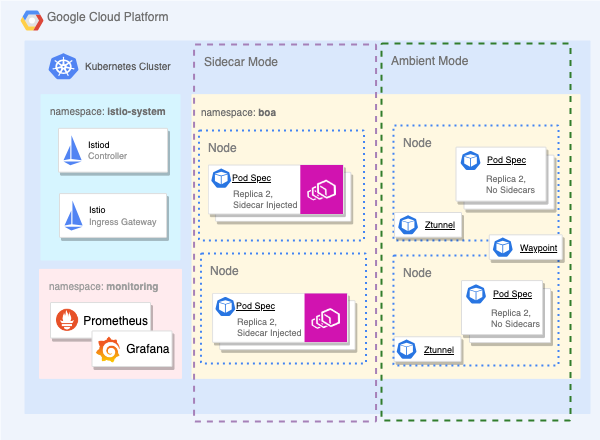
\includegraphics[width=1.0\linewidth]{resources/single-ns-test-infra.drawio.png}
    \caption{GCP Infrastructure Architecture with Single Namespace}
    \label{method:singleNsInfraArch}
\end{figure}

On the other hand, Figure \ref{method:multiNsInfraArch} shows the GCP infrastructure visualization of multiple namespace deployment (\cite{multiNsArticle}) of \acrshort{boa} application. The diagram shows up to 3 namespace deployment to keep the complexity of the figure lower however in the actual test 8 namespaces are used, each namespace representing a single microservice. In multiple namespace deployment environment, 'istio-system' and 'monitoring' namespaces remain unchanged but the data plane components of Istio are changed marginally. A Ztunnel is deployed per node wise whereas instance of Waypoint proxy is seen multiple times to cover multiple namespaces.
\begin{figure}[ht!]
    \centering
    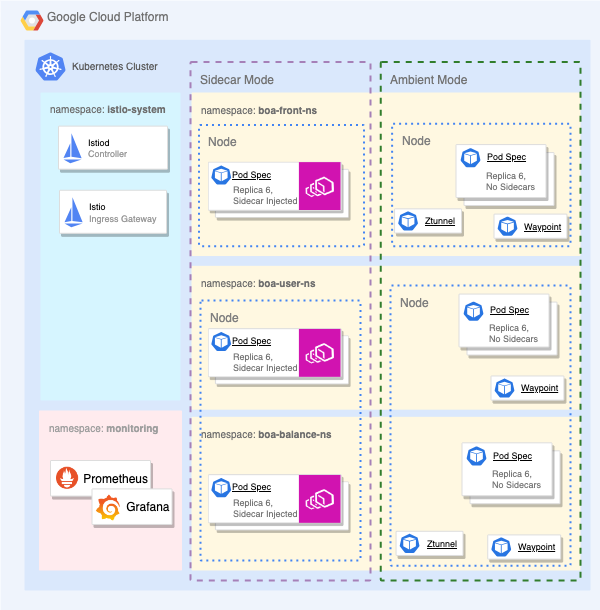
\includegraphics[width=1.0\linewidth]{resources/multi-ns-test-infra.drawio.png}
    \caption{GCP Infrastructure Architecture with Multiple Namespaces}
    \label{method:multiNsInfraArch}
\end{figure}


\subsubsection{Operational Complexity Measurement}
On a live Kubernetes cluster with hundreds or thousands of microservices, upgrading Istio becomes a challenge. Istio upgrades are important to avoid any vulnerabilities hence Istio documentation (\cite{istioDocCanaryUpgrade}) recommends a safe way of upgrading by using blue-green and canary deployment strategies to roll out new versions. Even though these methods are used pod restart is inevitable as the sidecar does not upgrade when the injector is upgraded rather, all injected pods must be restarted for their sidecars to upgrade. Hence a multiple Istio version deployment is made side by side by using Istio revision and tagging features (\cite{postaIstio2021}). By this not only the pods can switch to Istio versions dynamically with a restart, the ingress gateways can also be switched with zero downtime. To achieve the desired blue-green deployment a Kubernetes load balancer is used and Istio ingress gateway service types are set to ClusterIP to avoid creating further load balancer services.

\begin{figure}[ht!]
  \centering
  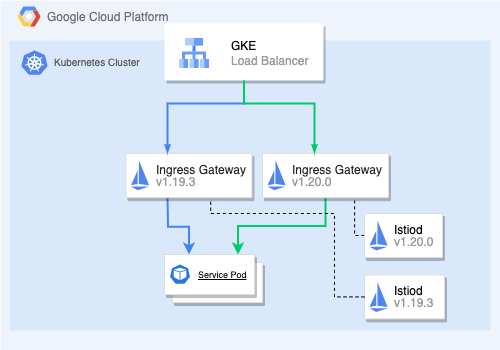
\includegraphics[width=1.0\linewidth]{resources/istio-upgrade-strategy.drawio.png}
  \caption{GCP Infrastructure Architecture of Istio Upgrade}
  \label{method:istioUpgradeArch}
\end{figure}

The upgrade architecture shown in Figure \ref{method:istioUpgradeArch} is heavily dependent on Istio Canary Deployment feature (\cite{istioDocHelm}). Istio version 1.18.5 is used a stable or blue version whereas version 1.19.3 is used as green version. Istio operator installation method is chosen for this test as it provides a greater control over parallel deployment instances of Istio.

Further to the Istio upgrade test, a no mesh to service mesh transition is also tested. When Istio is installed post application deployment on a Kubernetes cluster a restart of deployment is required for each namespaces. In sidecar mode, a Kubernetes object MutatingWebHookConfig acting as a webhook (\cite{krochmalski2017docker}) is deployed during Istio installation to track application pod creation and then to enable Istiod to inject a sidecar. All these pod detection and sidecar injection happens during pod initialization phase, hence if the Istio is installed after an application deployment Kubernetes admins always struggles to add Istio in the existing services. Fortunately, most of the times this is not a concern as in enterprise level, applications are deployed only after Kubernetes cluster is configured and validated with required elements including Istio. For academic purposes, this test checks whether ambient mode clears this blockers for cluster admins.

\subsection{Test Readiness}
\label{testReadiness}
Istio remains the core part of this research and to produce the research report on ambient mesh this paper explores the performance and operational complexity of Istio ambient mode. However, to test Istio from a real life cloud deployment environment, a deep dive into demo application deployment, Istio configuration and verification is required for a successful research result. In this section how Istio is installed, configured and verified is discussed along with \acrshort{boa} application set.

Istio documentation (\cite{istioDocInstall}) refers different methods for installing Istio system on a Kubernetes cluster however the preferred way is to use Istioctl - a tool which is installed on local system and uses Helm charts internally to install Istio on remote Kubernetes cluster. However for the Istio upgrade test the direct helm chart method is used in this research to use blue-green deployment. Istioctl comes with a lot of additional benefits like quick deployment of an ingress gateway or monitoring tool installation for testing purposes. In this research, Istio is installed and uninstalled several times using Istioctl and Helm Charts to capture test results. While using Istioctl, mainly two predefined profiles 'default' and 'ambient' is passed as command line argument to install Istio on remote cluster. A clean installation of Istio brings up two core components of Istio, Istiod - the control plane and the ingress controller in 'istio-system' namespace. These remains valid for both sidecar and ambient modes without any differences. Figure \ref{method:istioStdInstalledView} shows the cluster pod view from K9S - a tool used in all the tests to verify and query Kubernetes cluster components.

\begin{figure}[ht!]
    \centering
    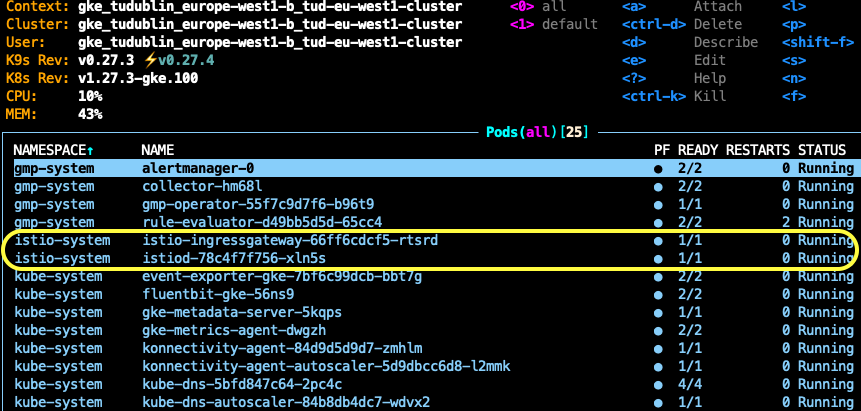
\includegraphics[width=1.0\linewidth]{resources/istio-std-installed.png}
    \caption{K9S View of Istio Control Plane}
    \label{method:istioStdInstalledView}
\end{figure}

The ingress gateway is used to serve the frontend microservice over public IP address whereas the Istiod configures all the sidecar proxies, Ztunnels and Waypoint proxies wherever these are application. 

A load testing script written in Python with Locust framework (\cite{locustDoc}) is used which comes by default as a microservice with \acrshort{boa} project. However, for this research project, some parameters of the script is modified and used from local test machine to simulate the live traffic to \acrshort{boa} application. With each tests, 50 user traffic is simulated at a rate of 1 per second for 10 minutes to perform sign up, login, transaction and logout operations.

\begin{figure}[ht!]
  \centering
  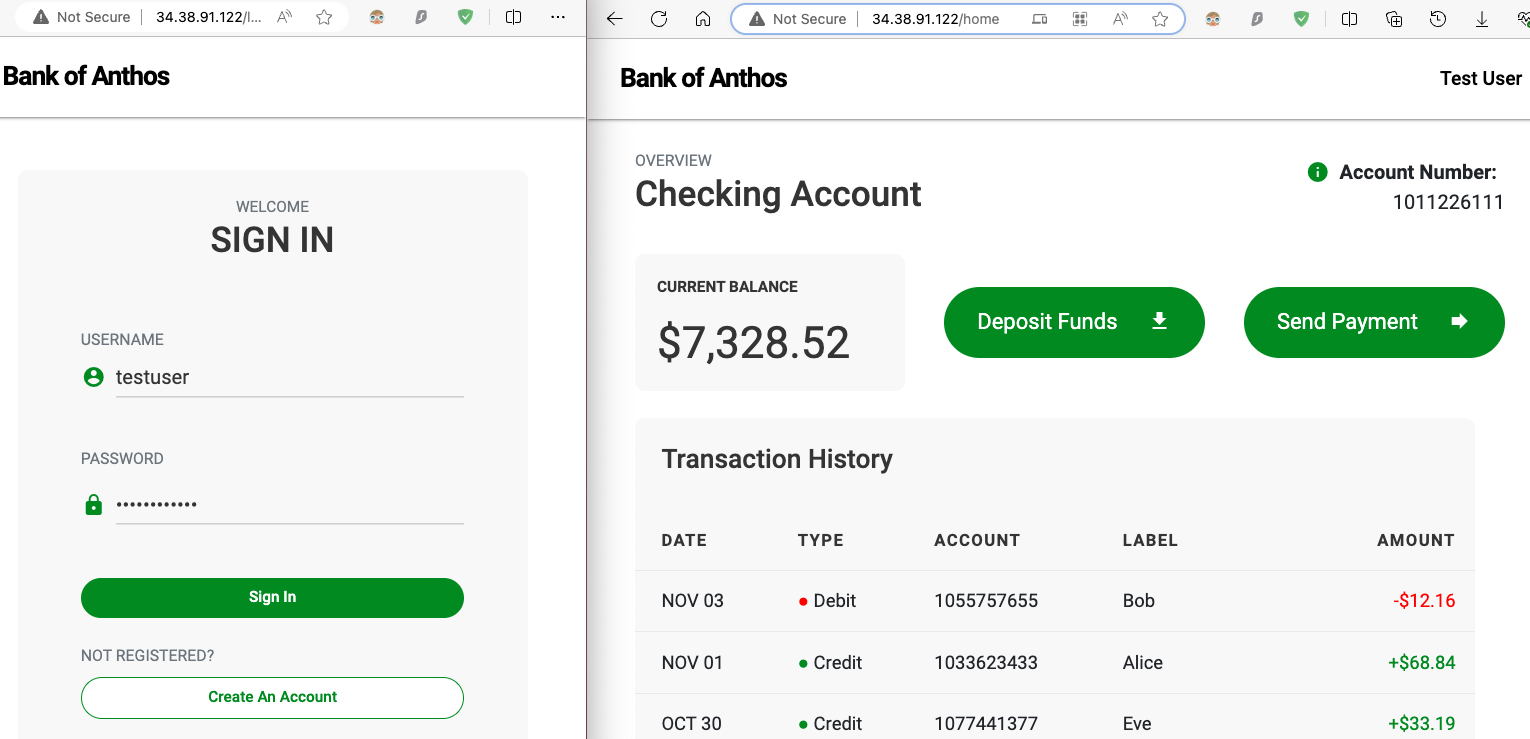
\includegraphics[width=1.0\linewidth]{resources/boa-view.png}
  \caption{Bank-of-anthos is accessible over external load balancer}
  \label{method:boaWebView}
\end{figure}

Figure \ref{method:boaWebView} shows the frontend view of the \acrshort{boa} application when it is accessed over public IP address. For some small test verifications a manual UI navigation method is also used by navigating to different pages of \acrshort{boa}.


\subsubsection{Sidecar Mode Test Setup}
With the \acrshort{gke} cluster in place and the Istio system installed with Istioctl 'default' profile, istiod - the control plane and an ingress gateway controller is deployed to the 'istio-system' namespace. An application namespace 'boa' is created for single namespace deployment test and 8 different namespaces are created by the microservice manifest files in case of multiple namespace deployment scenario. Namespace labelling is done with 'istio-injection=enabled' to configure the Istio control plane for injecting sidecars into microservice pods. For the \acrshort{boa} application deployment, first the JSON web token is deployed to 'boa' namespace as a ConfigMap followed by applying microservice manifests files. Accounts DB and Ledger DB microservices are deployed as StatefulSet whereas rest of the microservices are deployed as Kubernetes Deployment object. Once everything is successfully deployed, the K9s view shows all microservice pods with two replicas each in case of single namespace deployment and six replicas in case of multiple namespace deployment. As part of the verification process the pod descriptions are checked using K9s which reveals the sidecar container as 'istio-proxy' as shown in Figure \ref{method:istioSidecarInjectionView}.

\begin{figure}[ht!]
  \centering
  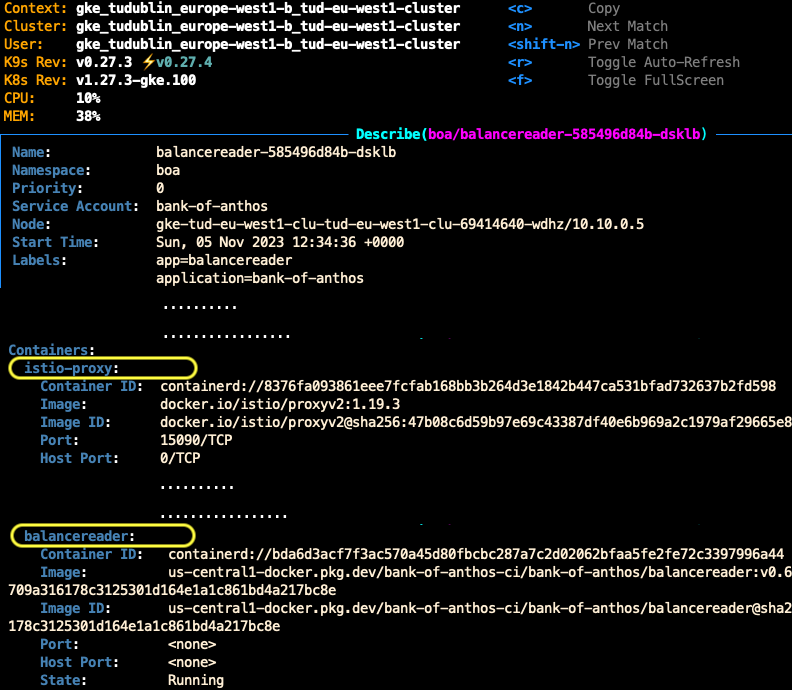
\includegraphics[width=1.0\linewidth]{resources/istio-sidecar-injection.png}
  \caption{Istio sidecar injection is in action}
  \label{method:istioSidecarInjectionView}
\end{figure}

In order to access the frontend microservice over a public IP address, a frontend gateway is attached to the istio ingress controller. By browsing to external IP address of the istio ingress controller, the \acrshort{boa} application is accessible from local system which confirms the application deployment. At this point, a verification is done whether Istio data plane is engaged in offering the basic service mesh functionality like mTLS encryption. Wireshark, a well known tool for packet sniffing is used on local system with kubectl plugin ksniff to intercept network packets between 2 microservices, frontend and balance reader. This verification involves a two stage process where the microservices are deployed previously on the cluster without Istio and the current deployment with Istio sidecar mode. While comparing the Wireshark captures for both cases, a balance value of "71580" is shown in plain text in case of no mesh set up. The plain text value is shown in Figure \ref{method:plainTxtWiresharkView} when Istio is not deployed.

\begin{figure}[ht!]
  \centering
  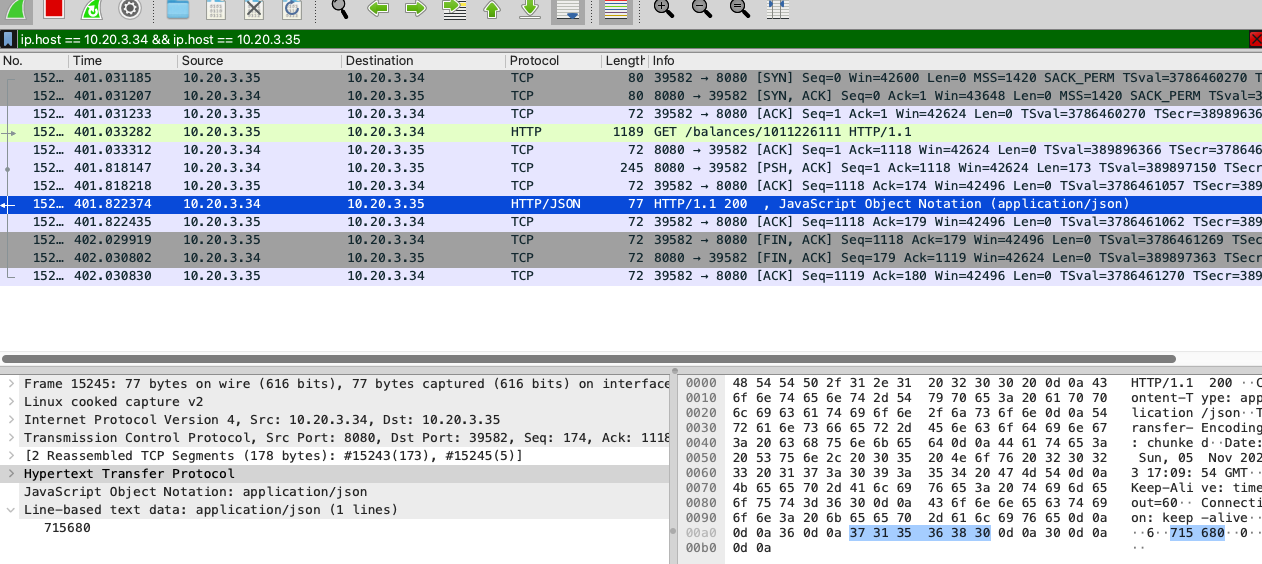
\includegraphics[width=1.0\linewidth]{resources/raw-balance-value.png}
  \caption{Plain Text Inter-Service Communication in No-Mesh Mode}
  \label{method:plainTxtWiresharkView}
\end{figure}

In single namespace test environment, 16 pods are running where:
\begin{itemize}
  \item Two replicas of eight microservices running a total of 16 sidecars
  \item Three cluster nodes are used to host 16 pods
\end{itemize}

In multiple namespace test environment the pod counts are 48 where:
\begin{itemize}
  \item Six replicas of eight microservices running 48 sidecars
  \item Eight cluster nodes are used to host 48 pods
\end{itemize}


\subsubsection{Ambient Mode Test Setup}
Ambient mode of Istio is installed using Istioctl, similar to sidecar mode but with a different profile named 'ambient'. This installation creates the istio-system namespace and deploys istiod control plane along with CNI plugin. Once the Istiod control plane is provisioned it spawns Ztunnel proxy pods on each running nodes. An Ingress controller is also used here and the frontend gateway is attached to it. The process of namespace labelling remains same but with a different key value pair of "istio.io/dataplane-mode=ambient". Though the majority of set up process remains same like sidecar mode, the verification process is different. To check the Ztunnel engagement, a handful traffic is sent to \acrshort{boa} by using the load generator script and packet sniffing is done for one of the microservice pod and a Ztunnel pod. The following two figures shows how the traffic is first intercepted by Ztunnel and then passed to the microservice pod. A closer look to Figure \ref{method:ztunnelLogView} and \ref{method:ztunnelTraceView} shows that Ztunnel received the traffic from ingress gateway 10.20.0.22 and then passing to the respective service pods.

\begin{figure}[ht!]
  \centering
  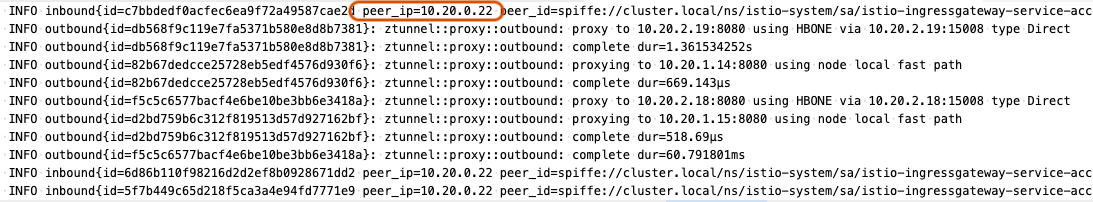
\includegraphics[width=1.0\linewidth]{resources/ztunnel-log.png}
  \caption{Ztunnel Pod Receiving Traffic}
  \label{method:ztunnelLogView}
\end{figure}

\begin{figure}[ht!]
  \centering
  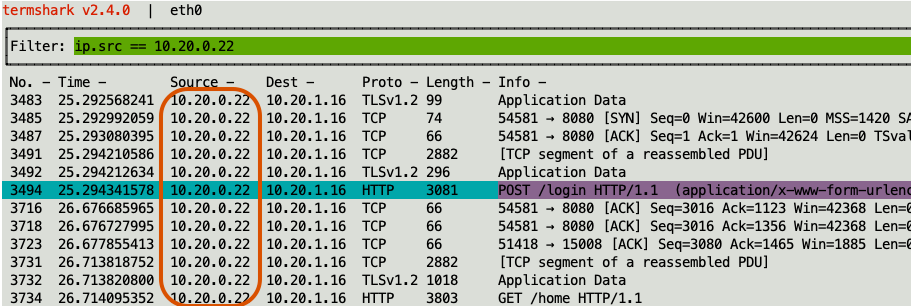
\includegraphics[width=1.0\linewidth]{resources/ztunnel-network-trace.png}
  \caption{Ztunnel Forwards Traffic to Microservice Pod}
  \label{method:ztunnelTraceView}
\end{figure}

To install the layer 7 proxy Waypoint Kubernetes gateway API CRDs are required to be installed on cluster as by default CRDs are not available with Istio installation. After configuring the custom CRDs required for Waypoint, each namespace gets a Waypoint proxy pod. When all microservices are deployed in a single namespace mapped there get a single Waypoint proxy but when the microservices are deployed across multiple namespaces, Waypoint proxies are deployed to each one of them. A comparison between Waypoint proxies deployed in single and multiple namespaces remains a crucial part of this research as it illustrates some most common real life deployment scenario where microservices are deployed in different namespaces. Figure \ref{method:waypointAppliedView} shows how the Waypoint proxy is engaged in ambient mesh setup to the microservice pods.

\begin{figure}[ht!]
  \centering
  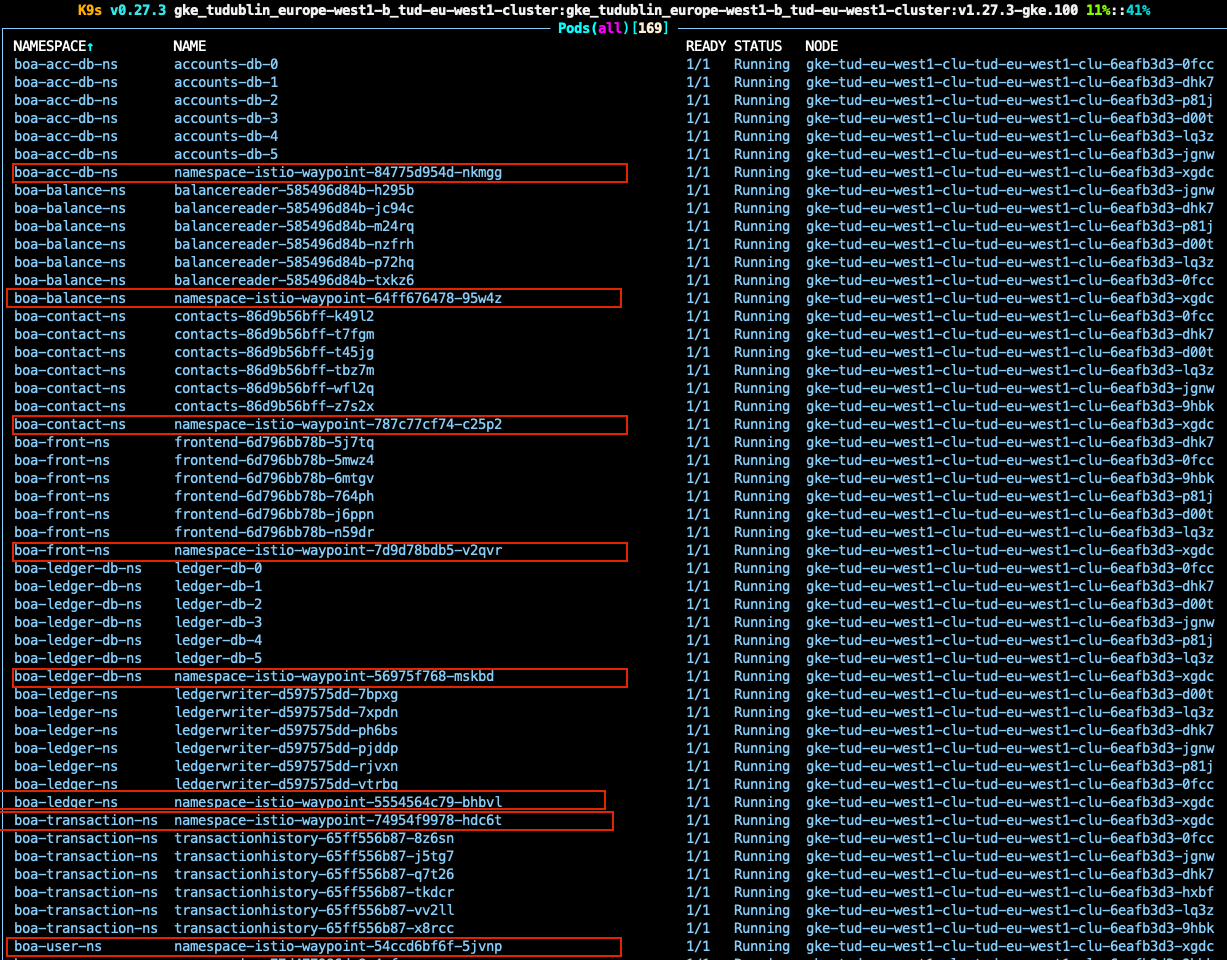
\includegraphics[width=1.0\linewidth]{resources/ambient-multi-ns-l4-l7-deployed.png}
  \caption{Waypoint Proxy is Applied Per Namespace Wise}
  \label{method:waypointAppliedView}
\end{figure}

To engagement Waypoint proxy, a L7 policy (Appendix \ref{appendix:waypoint}) is applied to return a direct response from the balance reader microservice. For the research purpose a simple HTTP filtering is done based on the host name where all the requests made to balance reader microservice will result in a HTTP 503 error. The L7 policy is applied via a Kubernetes manifest file and it is targeted to application namespace. Multiple namespace test scenario applies this policy to the balance reader namespace only. As the frontend is not able to get the balance value from balance reader microservice a '---' is displayed as shown in Figure \ref{method:l7PolicyAppliedView} when accessing \acrshort{boa} from a browser. This implies the traffic flows from istio ingress to host level Ztunnel proxy and finally followed by the Waypoint proxy before reaching to balance reader microservice.
To see Waypoint proxy engagement, a L7 policy (Appendix \ref{appendix:waypoint}) is applied to return a direct response from the balance reader microservice. For the research purpose a simple HTTP filtering is done based on the host name where all the requests made to balance reader microservice will result in a HTTP 503 error. The L7 policy is applied via a Kubernetes manifest file and it is targeted to application namespace. Multiple namespace test scenario applies this policy to the balance reader namespace only. As the frontend is not able to get the balance value from balance reader microservice a '---' is displayed as shown in Figure \ref{method:l7PolicyAppliedView} when accessing \acrshort{boa} from a browser. This implies the traffic flows from istio ingress to host level Ztunnel proxy and finally to Waypoint proxy before reaching to balance reader microservice.

\begin{figure}[ht!]
  \centering
  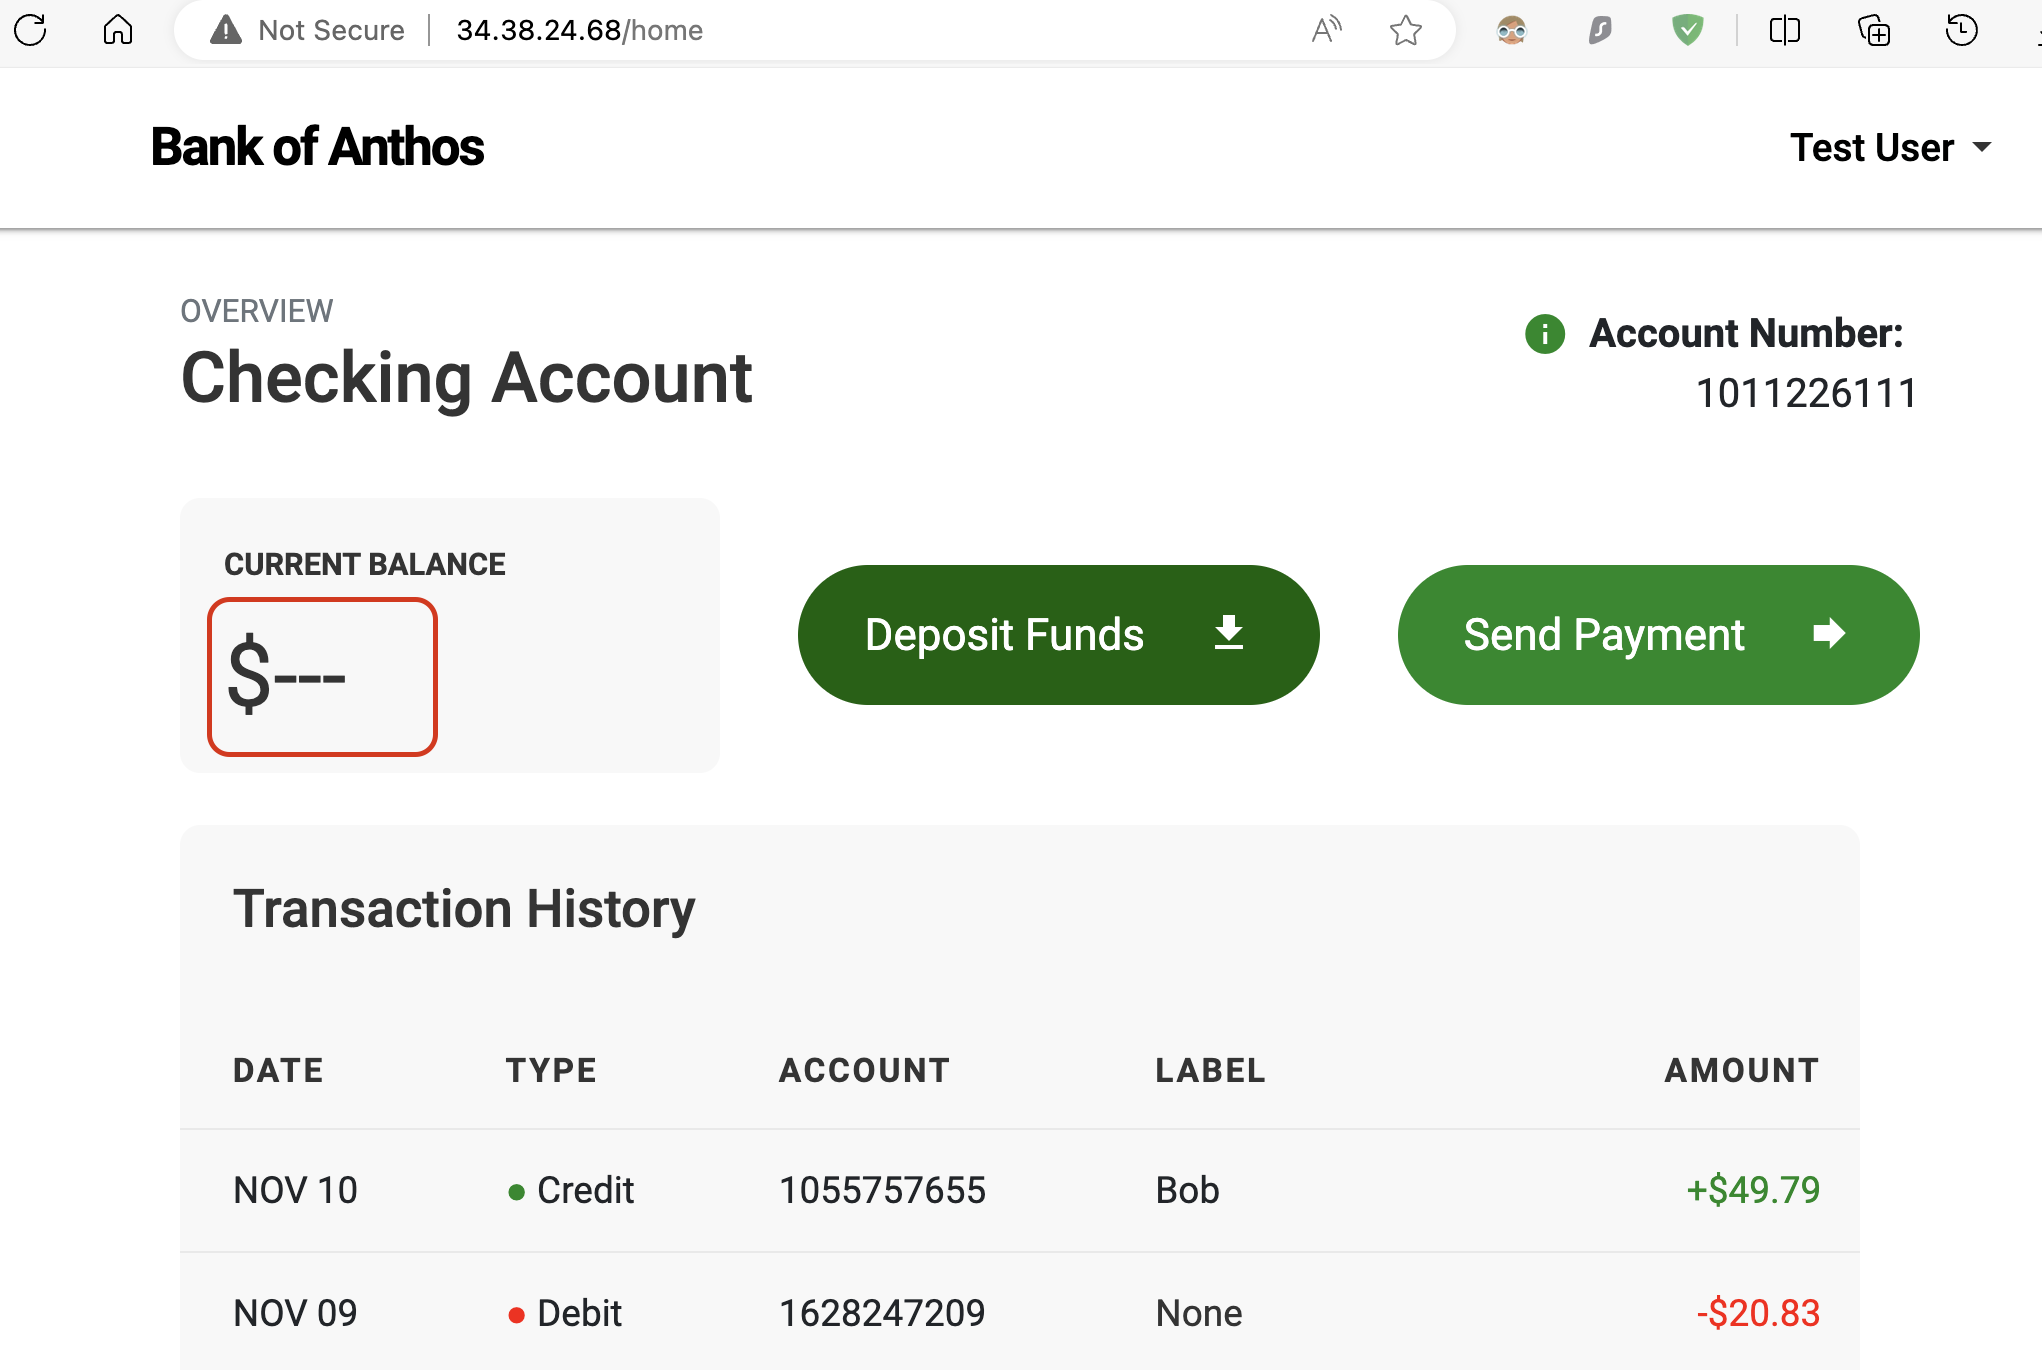
\includegraphics[width=0.7\linewidth]{resources/l7-policy-applied.png}
  \caption{Waypoint L7 Policy Reflecting on Frontend}
  \label{method:l7PolicyAppliedView}
\end{figure}

In single namespace test environment the pod count is 16 where:
\begin{itemize}
  \item Two replicas of eight microservices running without any sidecars
  \item Two Ztunnel proxy pods on 2 nodes
  \item One Waypoint proxy pod in the single namespace
\end{itemize}

In multiple namespace test environment the pod count is 48 where:
\begin{itemize}
  \item Six replicas of eight microservices without any sidecars
  \item Nine cluster nodes are used to host 48 pods
  \item Eight Waypoint proxy pods are deployed in 8 namespaces to support L7 processing
\end{itemize}

\subsubsection{Istio Upgrade Test Setup}
For Istio upgrade a different strategy is applied than testing Istio for performance benchmarking. The process involves deploying Istio operator - a program in the cluster to manage the state of Istio deployments. Istio operator manifest files come by default with Istioctl package but a custom resource definition or operator specification is made to configure the Istio control plane deployment. To deploy multiple versions of Istio on the same cluster, each version of Istioctl needs to be downloaded on the local system. The helm chart manifest files are applied to the cluster using 'kubectl' to deploy the operator. Once the operator is live on the cluster, the operator specification is applied to setup the Istiod control plane. This specification defines the Istio profiles to be installed on the cluster, which is 'minimal' and 'ambient' for sidecar and ambient mode respectively. By default the operator specification deploys an ingress gateway as well but that is restricted in the configuration to create manually in next stage. To verify the Istiod deployment state and whether multiple versions are running side by side on the cluster a kubectl describe pod command is used as shown in Figure \ref{method:multiIstiodVersions}.

\begin{figure}[ht!]
  \centering
  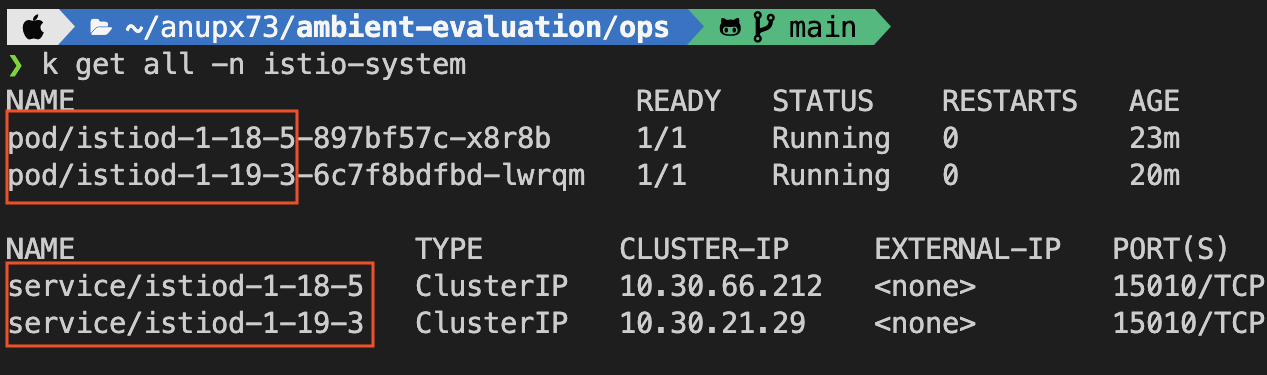
\includegraphics[width=1.0\linewidth]{resources/multi-istiod.png}
  \caption{Multiple Versions of Istiod is Live on Cluster}
  \label{method:multiIstiodVersions}
\end{figure}

Similarly, the ingress gateways are also deployed to the cluster with a defined configuration (Appendix \ref{appendix:researchRepo}) where the service type is set to ClusterIP to enable the ingress gateway service to maintain a local cluster IP address. As shown in Figure \ref{method:multiGateways} two Istio gateways are operating with different revisions and one of them are selected by the external Kubernetes load balancer to route the traffic.

\begin{figure}[ht!]
  \centering
  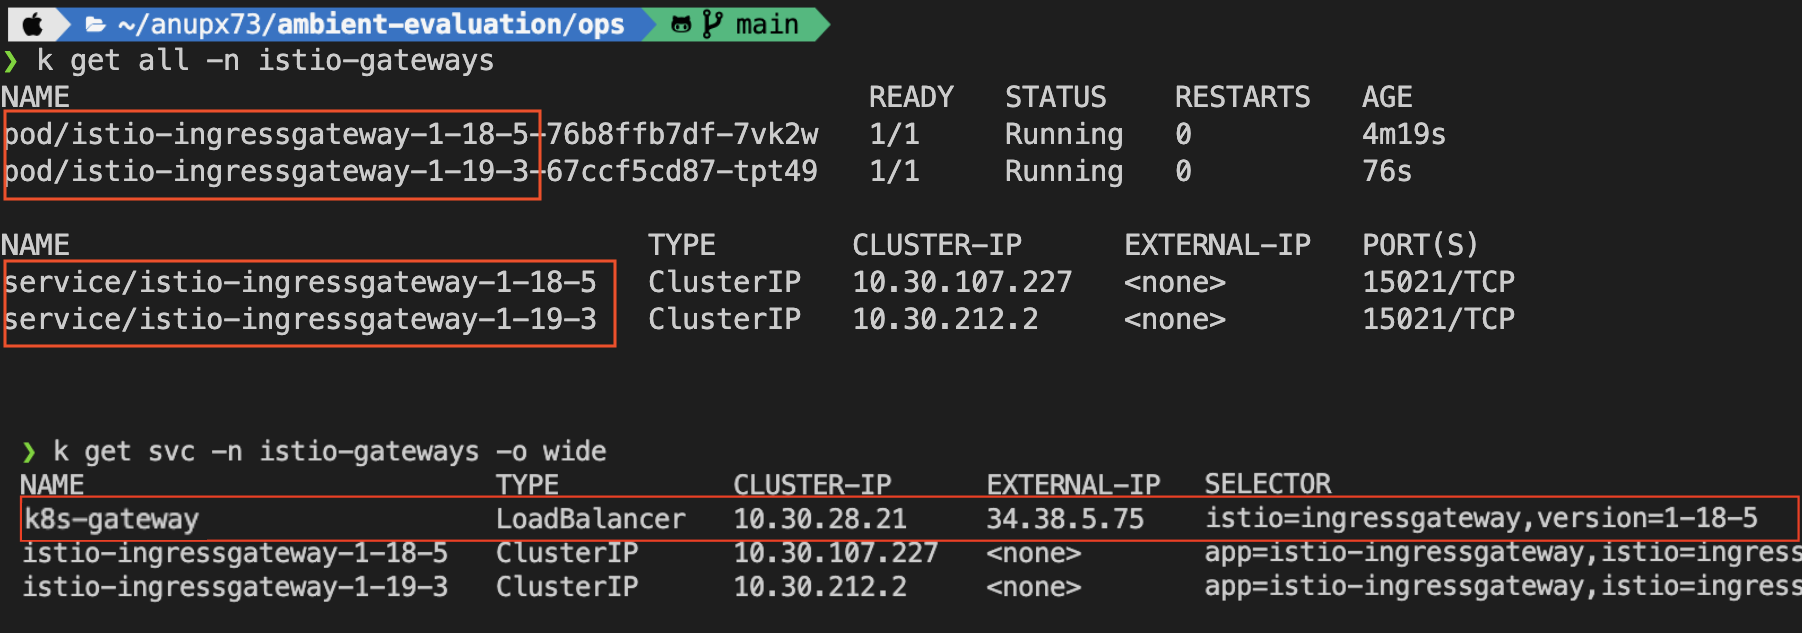
\includegraphics[width=1.0\linewidth]{resources/multi-gateways.png}
  \caption{Multiple Versions of Ingress Gateways and Load Balancer}
  \label{method:multiGateways}
\end{figure}

\subsection{Challenges Encountered}
\subsubsection{Ztunnel Blocks Service Start}
While setting up Istio with ambient mode, couple of microservices pods were stuck in Running state till the Ztunnel pod on the specific node was restarted. The configuration was:

\begin{itemize}
\item Istio with ambient profile installed on 3 nodes
\item 1 replica of all 8 microservices were deployed to a single node
\item Microservice deployment was done post Istio installation and namespace labelling
\end{itemize}

This scenario was not reproducible quite often, but this may need a further investigations into application configuration before flagging as a ambient mesh.

\subsubsection{Grafana Cloud Integration}
Grafana Cloud was chosen at first as a monitoring platform to retain research test data for a long period of time. After the Grafana cloud integration with the GKE instance was made, a few tests were done with Istio system data capture. This resulted in exceeding the free-tier metric limit of 10000 per month by 400\%. Later, the metric ingestion limit was controlled up to a certain limit by adding a filter in the Prometheus remote data export configuration; however, to avoid any unforeseen issues, switching to a Grafana local instance was preferred. Appendix \ref{appendix:grafana} mentions the details about setting up Grafana cloud integration.